\documentclass{article}
\usepackage{tikz}

\begin{document}

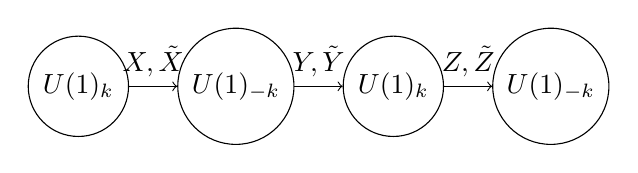
\begin{tikzpicture}[node distance=2cm]
    \node[draw,circle] (U1) {$U(1)_k$};
    \node[draw,circle] (U2) [right of=U1] {$U(1)_{-k}$};
    \node[draw,circle] (U3) [right of=U2] {$U(1)_k$};
    \node[draw,circle] (U4) [right of=U3] {$U(1)_{-k}$};

    \draw[->] (U1) -- node[above] {$X,\tilde{X}$} (U2);
    \draw[->] (U2) -- node[above] {$Y,\tilde{Y}$} (U3);
    \draw[->] (U3) -- node[above] {$Z,\tilde{Z}$} (U4);
\end{tikzpicture}

\end{document}